\documentclass[11pt,a4paper]{article}

% ------------------------------------------------------------
% Packages
% ------------------------------------------------------------
\usepackage[utf8]{inputenc}
\usepackage[T1]{fontenc}
\usepackage{newtxtext}
\usepackage{newtxmath}
\usepackage{microtype}
\usepackage[margin=2.5cm]{geometry}
\usepackage{setspace}
\usepackage{parskip}
\usepackage{graphicx}
\usepackage{float}
\usepackage{amsmath, amssymb}
\usepackage{booktabs}
\usepackage{array}
\usepackage{xcolor}
\usepackage{hyperref}
\usepackage{titlesec}
\usepackage{caption}
\usepackage{enumitem}
\usepackage{fancyhdr}
\usepackage{longtable}
\usepackage{url}
\setlength{\parindent}{0pt}

% ------------------------------------------------------------
% Hyperlinks and layout
% ------------------------------------------------------------
\hypersetup{
    colorlinks=true,
    linkcolor=blue!50!black,
    urlcolor=blue!50!black,
    citecolor=blue!50!black
}

\setstretch{1.03}
\setlength{\parindent}{0pt}
\setlength{\parskip}{0.2em}

\definecolor{titleblue}{RGB}{27, 58, 99}
\definecolor{softgray}{RGB}{245, 245, 245}
\definecolor{softred}{RGB}{180, 50, 50}

\titleformat{\section}
  {\large\bfseries\color{titleblue}}
  {\thesection.}{0.6em}{}

\titleformat{\subsection}
  {\normalsize\bfseries\color{titleblue}}
  {\thesubsection.}{0.6em}{}

\pagestyle{fancy}
\fancyhf{}
\fancyhead[L]{Bioinformatics Article Summary}
\fancyhead[R]{Hierarchical marker genes selection in scRNA-seq analysis}
\fancyfoot[C]{\thepage}

% ------------------------------------------------------------
% Useful commands
% ------------------------------------------------------------
\newcommand{\todochange}[1]{\textcolor{softred}{[CHANGE: #1]}}

\newcommand{\missingfigurebox}[1]{%
\fbox{%
\begin{minipage}[c][4cm][c]{0.9\linewidth}
\centering
\textit{Figure file not found:} \texttt{#1}\\
Replace this box with the correct image file or keep it as a placeholder.
\end{minipage}}
}

\newcommand{\maybeincludefigure}[3]{%
\begin{figure}[H]
    \centering
    \IfFileExists{#1}{\includegraphics[width=#2]{#1}}{\missingfigurebox{#1}}
    \caption{#3}
\end{figure}
}

% ------------------------------------------------------------
% Document
% ------------------------------------------------------------
\begin{document}

\begin{titlepage}
    \centering
    \vspace*{2cm}
    {\Huge\bfseries\color{titleblue} Hierarchical marker genes selection in scRNA-seq analysis\par}
    \vspace{0.4cm}
    {\LARGE Article Summary and Robustness Analysis\par}
    \vspace{1cm}
    {\large Bioinformatics / scRNA-seq review\par}
    \vspace{1.5cm}

    \begin{minipage}{0.9\textwidth}
    \centering
    \setlength{\fboxsep}{12pt}
    \colorbox{softgray}{
        \parbox{0.85\textwidth}{
        \textbf{Article reference:} Sun, Y. \& Qiu, P. (2024). \textit{Hierarchical marker genes selection in scRNA-seq analysis}. PLOS Computational Biology.\\[0.2cm]
        \textbf{Main idea:} The authors propose a hierarchical marker gene selection strategy to overcome limitations of the classical one-vs-all approach, especially when cell types are closely related and share marker genes.\\[0.2cm]
        \textbf{Code:} \url{https://github.com/jefgr/Bioinformatics}
        }
    }
    \end{minipage}

    \vfill
    {\large Jef Grupping and Coline Clerbaux \par}
    \vspace{0.4cm}
    {\large May 2026 \par}
    \vfill
\end{titlepage}

\tableofcontents
\newpage

% ------------------------------------------------------------
\section{Introduction}

Single-cell RNA sequencing (scRNA-seq) measures gene expression at the level of individual cells. Unlike bulk RNA sequencing, which averages expression over a population of cells, scRNA-seq makes it possible to study cellular heterogeneity and to distinguish cell types or cell states inside complex tissues.

However, scRNA-seq generates very large and complex datasets. One central challenge is therefore to identify marker genes, namely genes whose expression helps distinguish one cell type from another.
These marker genes are essential for annotating clusters obtained after unsupervised analysis and for giving them biological meaning.

One of the most common strategies for identifying marker genes is the "one-vs-all" approach. In this framework, one cluster is compared against all the other clusters combined, and genes that are significantly more expressed in that cluster are selected as markers.

This strategy is often used, but it has a large limitation: when several clusters are closely related cell types, the selected marker genes will often overlap.
They capture what these related clusters have in common rather than what truly distinguishes them.
As a result, the one-vs-all strategy may fail to separate similar cell types accurately and may reduce the interpretability of the results.

To address this issue, the authors propose a hierarchical marker gene selection method.

As shown in Figure ~\ref{fig:figure1}, in the heatmap of the classical Seurat one-vs-all, there is often a strong off-diagonal signal.
This is problematic, because diagonal blocks represent marker genes strongly expressed in their intended cluster.
Thus, off-diagonal blocks indicate that these marker genes are also strongly expressed in other clusters, which suggests poor specificity.

The hierarchical approach is thus a proposed improvement to reduce the off-diagonal signal.
It starts from all cell types grouped together, and then splits them progressively into smaller branches that are more specific.
At each split, marker genes are recalculated for the groups being separated at that level of the hierarchy.
The final result is a new heatmap (Figure~\ref{fig:figure1}),where marker genes are more specifically expressed in the expected clusters.. 

\begin{figure}[!htbp]
    \centering
    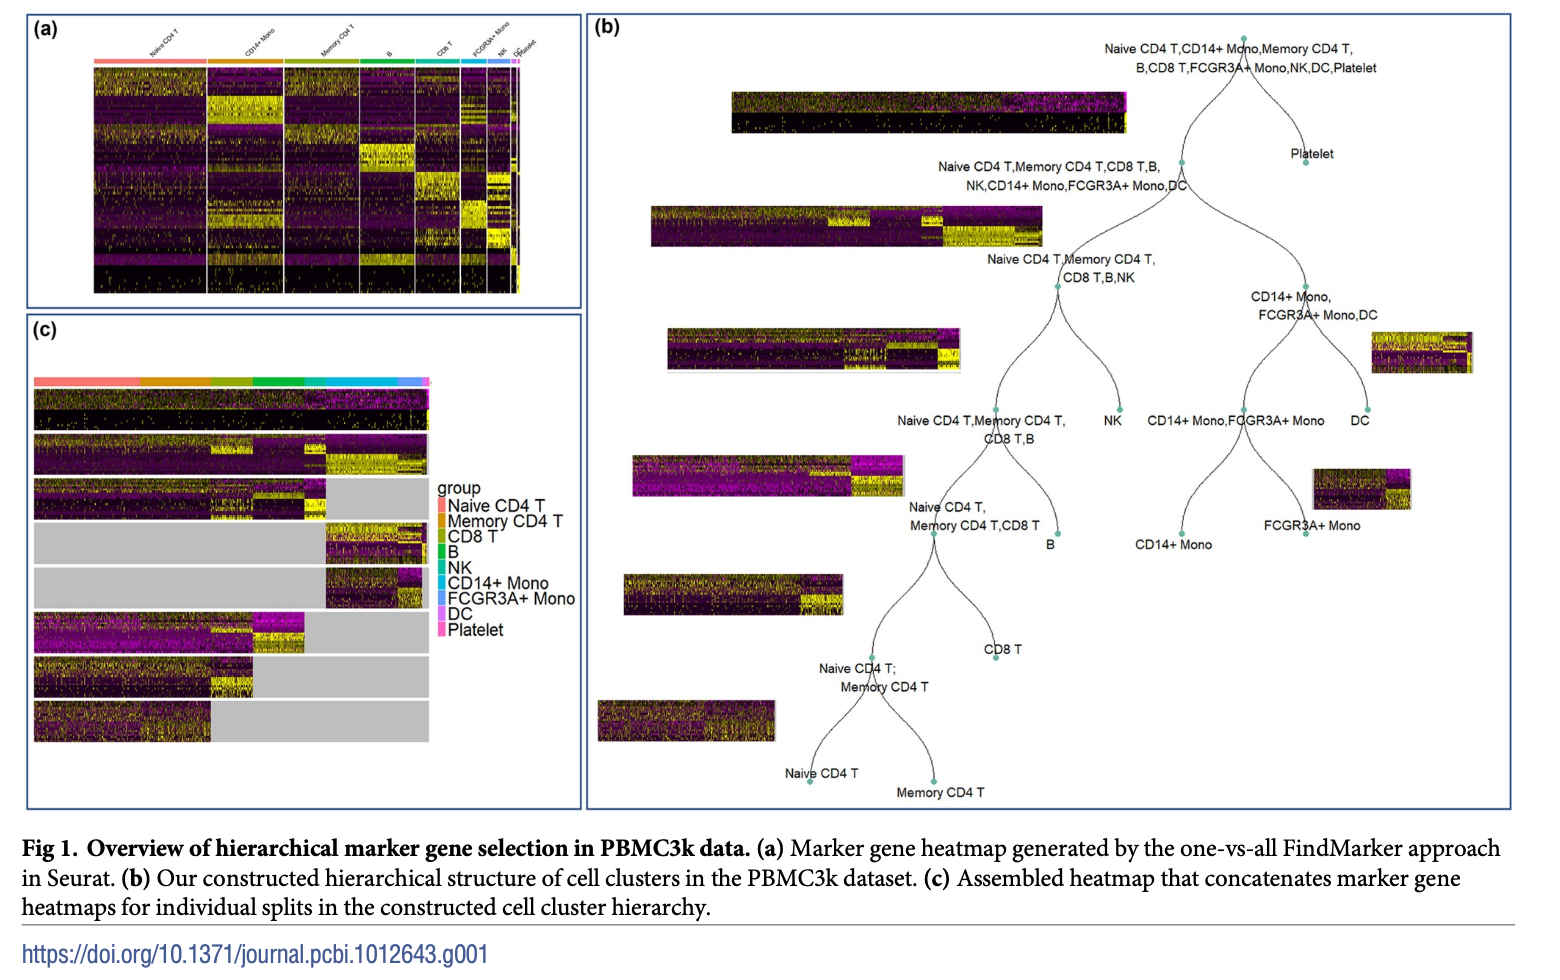
\includegraphics[width=\textwidth]{C1.png}
    \caption{}
    \label{fig:figure1}
\end{figure}


\section{The method}

\subsection{Input of the method}

The method of the article uses a preprocessed and clustered scRNA-seq dataset (a gene expression matrix, predefined cell clusters or annotated cell types and a marker gene heatmaps generated from one-vs-all marker selection). 

The goal of the method is not to discover clusters but to organise existing clusters into a hierarchy and select better marker genes for each level of that hierarchy. 

\subsection{Scoring function} 

To construct each split of the hierarchy, the authors use a score as a decision criterion to determine which groups should be merged or separated. The score is defined :

\[
 s = \frac{V_{\mathrm{diagonal}} - k \cdot V_{\mathrm{off-diagonal}}}{N_{\mathrm{celltypes}}}
\]

where:

\begin{itemize}[leftmargin=1.5em]
    \item $V_{\mathrm{diagonal}}$ measures the average expression in the diagonal blocks;
    \item $V_{\mathrm{off-diagonal}}$ measures the strongest undesirable off-diagonal expression;
    \item $N_{\mathrm{celltypes}}$ is the number of cell types or groups considered at that step;
    \item $k$ is a weight controlling how strongly off-diagonal expression is penalised.
\end{itemize}

The parameter $k$ is set at $5$. Reviewers of the article questioned this parameter because it could seem to be chosen arbitrarily.
In their response, the authors explained that they tested other values of k on the PBMC control dataset.
They compared $k=1$, $k=5$ and $k=7$ on the PBMC control dataset and observed that these values produced the same hierarchy.
Based on this result, they argued that the method is robust around the default value k=5.
They also tested an extreme case with a very small value, $k=0.01$.
In this case, some cell types were grouped with unrelated lineages, which means that the parameter choice can strongly affect the biological interpretation of the hierarchy.

However, the choice of $k=5$ remains mostly empirical.
They have shown that it works well on the PBMC control dataset, but they do not provide a general rule explaining how $k$ should be selected for a new dataset. 


\subsection{Hierarchy construction and assembled heatmap}

The hierarchy is constructed by repeatedly testing possible merges between clusters. 
For each merge, the method recalculates marker genes and evaluates the resulting heatmap with the scoring function. 
The merge is kept only if it improves the heatmap score.
When no merge improves the score, the current groups define a split, and the same process is repeated inside each branch.

After the hierarchy is constructed, the marker gene heatmaps from all splits are concatenated into one assembled heatmap, as you can see in the c part of Figure~\ref{fig:figure1}. Each horizontal block corresponds to one split of the hierarchy. This visualisation summarises which marker genes are selected at each level and whether they are specifically expressed in the expected cell groups.

\section{Datasets and comparisons in the article}

Sun and Qiu mainly evaluate the method on PBMC datasets.
This is a reasonable choice because PBMC data contain immune cell populations with meaningful relationships: T-cell subtypes, monocyte subtypes, B cells, NK cells, dendritic cells and platelets.
PBMC3k is used as the main illustrative example.
PBMC control and PBMC stimulated datasets are used for larger classification and cross-dataset mapping experiments.

The article compares hierarchical marker genes against several alternatives, including all genes, highly variable genes, Seurat one-vs-all marker genes and scGeneFit-based approaches.
The evaluation relies heavily on KNN classification: selected marker genes are used as features, and the classifier tests whether cells can be assigned to the correct cell type.

\begin{figure}[!htbp]
    \centering
    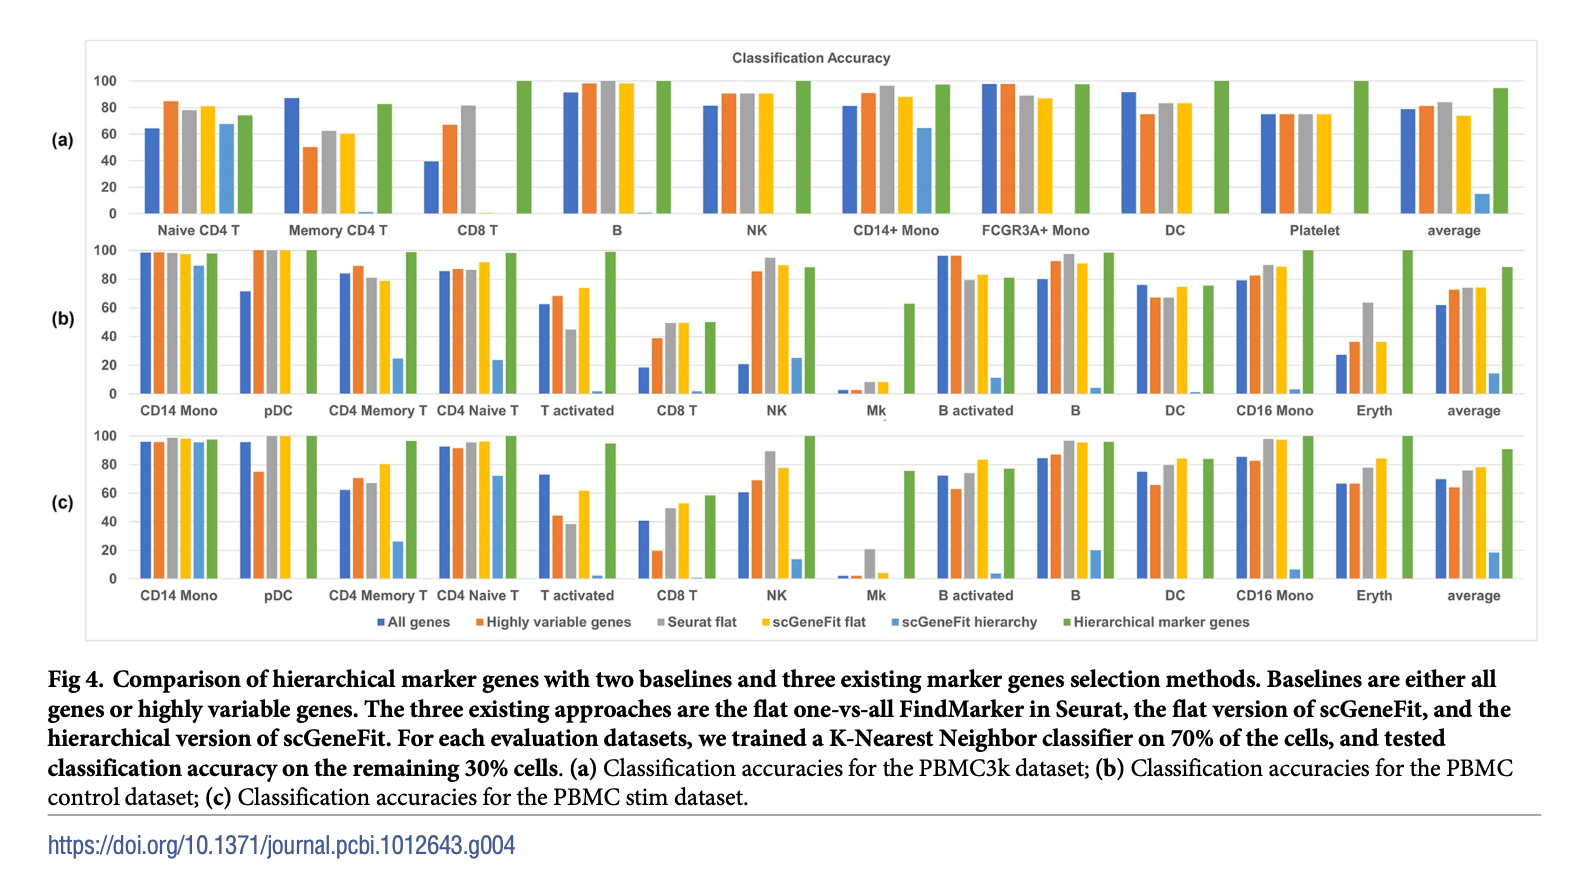
\includegraphics[width=0.75\textwidth]{C2.png}
    \caption{}
    \label{fig:fig2}
\end{figure}

For PBMC3k, the authors report that hierarchical marker genes improve classification accuracy by 10.5\% compared with Seurat one-vs-all marker genes, while using the same number of genes. For PBMC control, they report an average accuracy of 88\% with hierarchical marker genes, compared with 74\% for Seurat one-vs-all marker genes.

However, Figure~\ref{fig:fig2} suggests that the improvement is not systematic for every individual cell type.
In a few cases, Seurat flat is slightly above the hierarchical method, for example, Naive CD4 T in PBMC3k and NK or CD14 Mono in PBMC control.
This does not contradict the author's main result, but it shows that the advantage of the hierarchical method is mainly visible at the average level and for cell types that are difficult to separate.

This can be explained by the design of the method.
The hierarchical approach is most useful when cell types are closely related, because it selects marker genes at different levels of the hierarchy.
When a cell type is already relatively distinct, a classical one-vs-all comparison may already select efficient markers.
This may explain why Seurat flat can perform very well for some individual cell types.

The authors themselves discuss a stronger limitation with the pancreas dataset.
This dataset contains four clearly distinct cell types: alpha, beta, gamma, and delta cells.
In this case, merging clusters does not reduce the off-diagonal signal, so the algorithm stops at the first iteration and becomes equivalent to the flat one-vs-all approach.

Overall, the hierarchical method is not universally superior.
It is most useful when the data contain meaningful hierarchical structure, such as related immune cell lineages.
When cell types are already clearly separated, the method may add little information compared with a simpler one-vs-all strategy.


\section{Project question and experimental design}

The original article shows that the method improves marker gene selection in PBMC datasets. Our question is whether the results remain stable when marker selection parameters are modified.

In transcriptomics, marker genes are used to interpret biological differences between cell types.
Thus, if a small parameter change gives a similar hierarchy but different marker genes, the method may look stable visually while its biological interpretation remains sensitive to the choice of parameter.

%maybe add somthenig related to change of dataset ?
We also tested the method on additional datasets.
We did this to see if the method would hold up when the dataset was not selected with the method in mind.

\subsection{Parameters tested}

In our experiments, we keep the hierarchical method fixed, and we modify marker selection parameters.
We choose to modify two parameters:

\begin{itemize}[leftmargin=1.5em]
    \item $n$: the number of top marker genes retained for each group or split;
    \item $pct$: the minimum fraction of cells in which a gene must be expressed to be considered as a candidate marker.
\end{itemize}

These parameters directly affect the selected gene lists.
Increasing $n$ keeps more genes, which may help classification but can reduce interpretability.
Changing $pct$ changes which genes are eligible as markers: a low value is more permissive, while a high value is more restrictive.

The original PBMC3k setting is $n=10$ and $\texttt{pct}=0.25$.
Four additional settings were tested:
\begin{enumerate}
    \item $n=5,\ \texttt{pct}=0.25$
    \item $n=10,\ \texttt{pct}=0.10$
    \item $n=10,\ \texttt{pct}=0.50$
    \item $n=25,\ \texttt{pct}=0.25$
\end{enumerate}

For each setting, we compared the \texttt{hierarchy\_list} files to see whether the same hierarchy was recovered, and we compared the \texttt{hierarchy\_gene\_list} files with the original setting. 

To do that, we use Jaccard similarity:

\[
J(A,B) = \frac{|A \cap B|}{|A \cup B|}.
\]

This score measures the overlap between two marker gene sets.
A high Jaccard similarity means that the two settings selected similar marker genes.
A low value indicates that the selected genes changed more strongly. 

Then, we used the selected marker genes as features in a KNN classifier.
This allows us to test whether different marker gene lists still contain enough information to classify cell types correctly.

\subsection{Additional datasets}

We also looked at a different dataset to see if the hierarchical method could be used there.
For this we used a dataset with 1781 cells and 14818 genes from a study about Activin A in mice by Yin et al.\cite{yin2026}.
We will refer to this dataset as the Activin A dataset.
We ran the hierarchical method on this dataset with the parameters set at $n=10$ and $pct=0.25$.
We also tested the results using a KNN classifier.

\section{Results}

\subsection{Hierarchy stability}

Across the tested parameter settings, the hierarchy structure remained stable in our comparison of the hierarchy output files.
The same eight PBMC3k splits were recovered: Platelet versus the rest, monocytes versus the remaining groups, B/DC versus T/NK, NK versus T cells, CD8 T versus CD4 T, FCGR3A+ Mono versus CD14+ Mono, DC versus B, and Memory CD4 T versus Naive CD4 T.

This result supports one part of the original article: the broad PBMC3k hierarchy is robust under the marker selection parameter changes tested here.
However, this should not be overinterpreted.
Our test only covers a limited parameter range and one dataset.
It does not prove that the hierarchy would remain stable under different preprocessing choices, different clustering resolutions, different datasets or different values of the score parameter k.

\subsection{Marker gene instability and biological interpretation}

The stability of the hierarchy does not extend to the marker gene lists.
Table~\ref{tab:gene_counts} shows that the number of selected unique marker genes changes strongly across parameter settings, from 66 genes for $n=5$, $\texttt{pct}=0.25$ to 312 genes for $n=25$, $\texttt{pct}=0.25$.

\begin{table}[H]
\centering
\caption{Number of unique marker genes and classification results by parameter setting.}
\label{tab:gene_counts}
\begin{tabular}{lrrrr}
\toprule
Parameter setting & Unique genes & Mean KNN & SD KNN & Mean macro-F1 \\
\midrule
$n=5,\ \texttt{pct}=0.25$ & 66 & 0.826 & 0.009 & 0.859 \\
$n=10,\ \texttt{pct}=0.10$ & 135 & 0.824 & 0.011 & 0.868 \\
$n=10,\ \texttt{pct}=0.25$ & 127 & 0.863 & 0.011 & 0.891 \\
$n=10,\ \texttt{pct}=0.50$ & 127 & 0.864 & 0.012 & 0.893 \\
$n=25,\ \texttt{pct}=0.25$ & 312 & 0.868 & 0.011 & 0.889 \\
\bottomrule
\end{tabular}
\end{table}


% TODO Coline, should the mean and SD not have same amount of digits?

The Jaccard matrix in Figure~\ref{fig:Figure4} shows that several parameter settings share only a limited fraction of genes.
Compared with the reference setting $n=10$, $\texttt{pct}=0.25$, the Jaccard similarity is 0.52 for $n=5$, $\texttt{pct}=0.25$, 0.34 for $n=10$, $\texttt{pct}=0.10$, 0.32 for $n=10$, $\texttt{pct}=0.50$, and 0.41 for $n=25$, $\texttt{pct}=0.25$.

\begin{figure}[H]
\centering
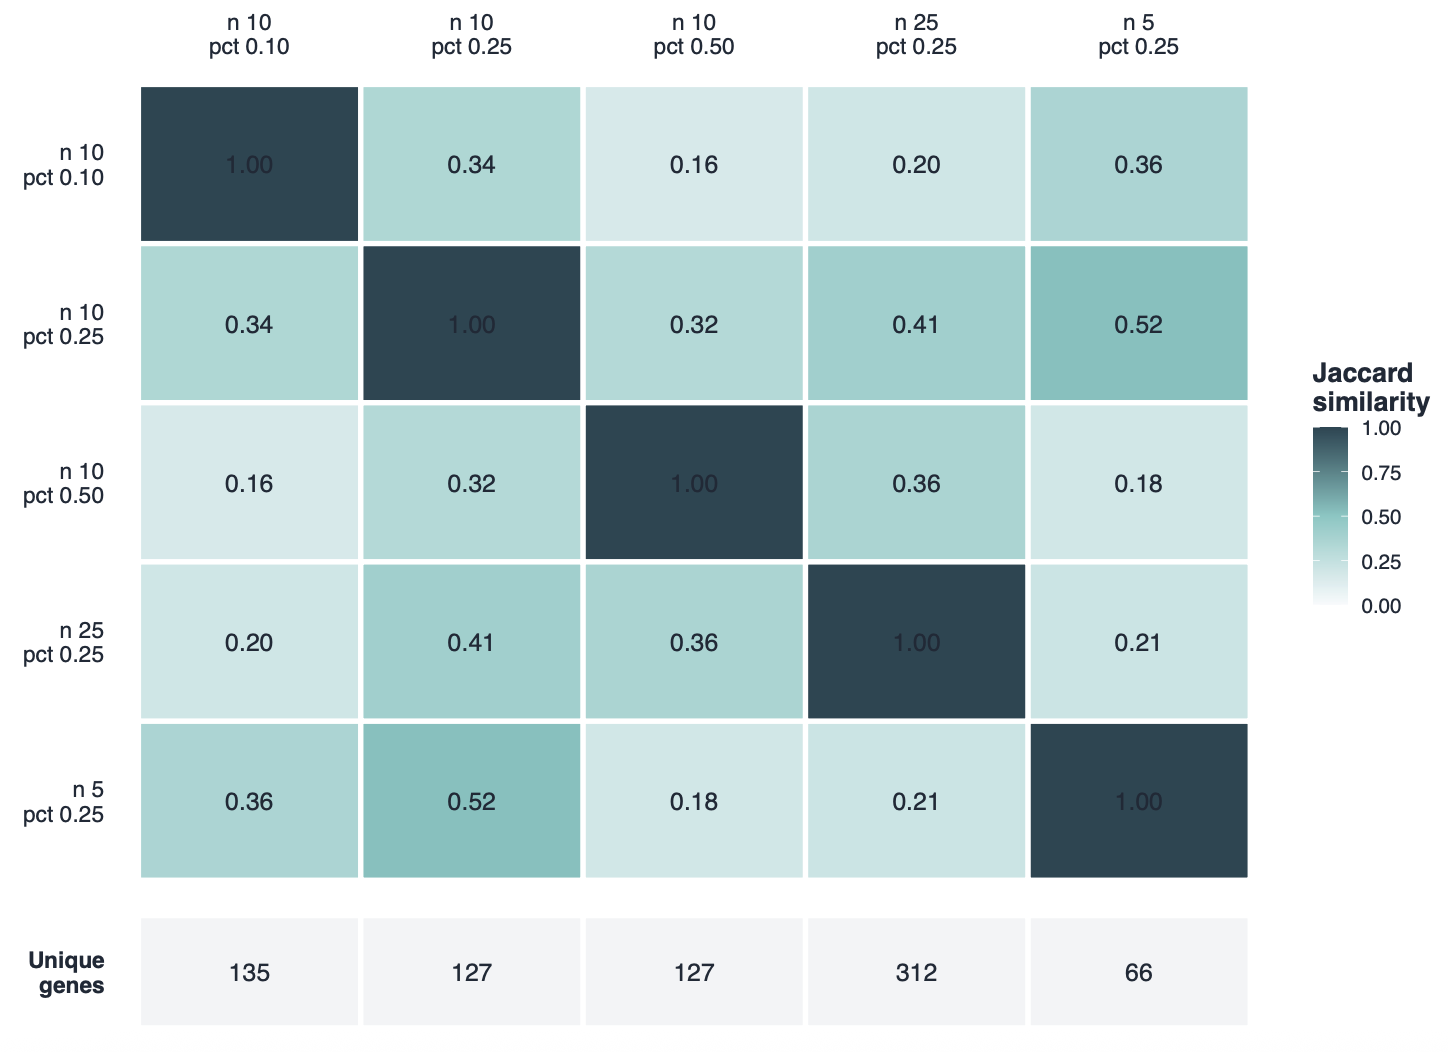
\includegraphics[width=0.5\linewidth]{C4.png}
\caption{Jaccard similarity between global marker gene lists.}
\label{fig:Figure4}
\end{figure}

The same hierarchy can be explained by different marker gene lists.
Marker genes are not only computational features; they are also used as biological evidence.
If the selected genes change substantially when parameters change, then the biological interpretation of a branch or cell type is less stable than the hierarchy list suggests.
% TODO coline, which visualisation do you mean here?

This analysis separates structural stability from explanatory stability. The split hierarchy may tell the same high-level story, but the molecular evidence used to support that story changes. This is especially important because marker genes can later be used for annotation, experimental validation, cytometry panels or biological interpretation. If a branch is stable but the markers supporting it are parameter-sensitive, then the branch may reflect a robust separation in expression space while the precise biological signature remains uncertain.

Marker genes act as compact biological signatures of cell identity. A good marker signature should not only allow good classification, but also remain stable and interpretable across reasonable parameter choices. Our Jaccard results suggest that the marker-gene signatures are more parameter-dependent than the hierarchy itself.



\subsection{KNN classification}

The KNN results show that marker gene instability does not necessarily lead to a large decrease in classification performance.
Several different gene lists classify cells with comparable accuracy.
As shown in Figure~\ref{fig:Figure3}, some parameter settings remain close in KNN accuracy even when their Jaccard similarity to the reference marker gene list differs substantially.

\begin{figure}[!htbp]
    \centering
    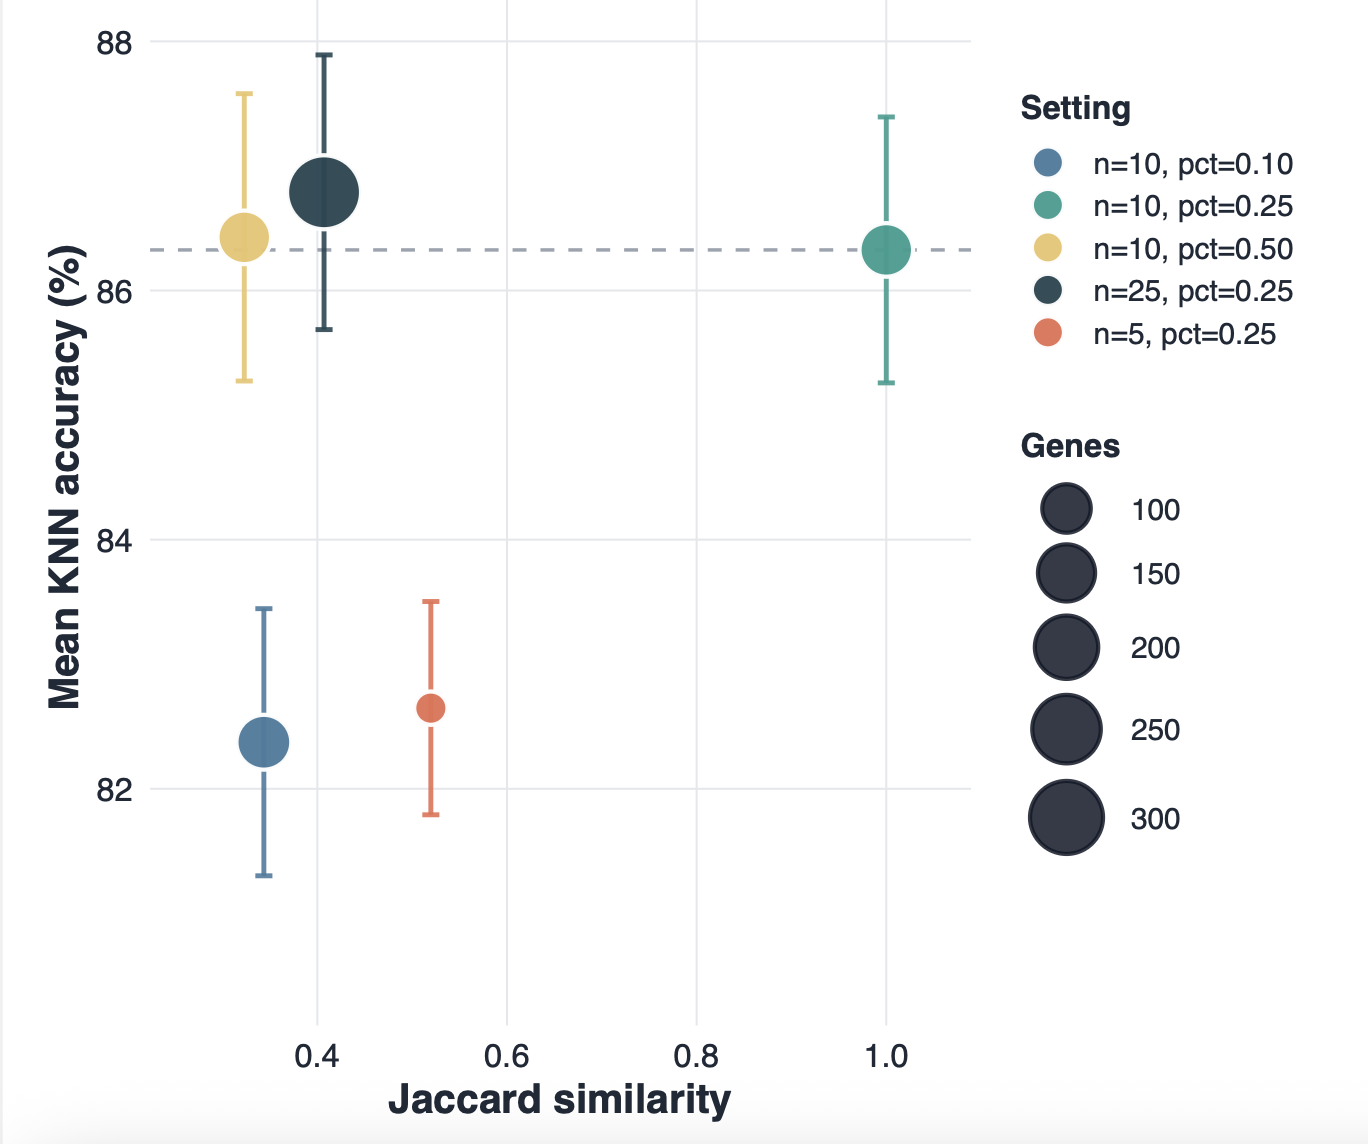
\includegraphics[width=0.50\textwidth]{C3.png}
    \caption{Relationship between marker gene stability and KNN classification performance}
    \label{fig:Figure3}
\end{figure}

For example, the settings $n = 10$, $pct = 0.25$, $n = 10$, $pct = 0.50$, and $n = 25$, $pct = 0.25$ reach similar mean accuracies of approximately 0.862, 0.864, and 0.868, respectively.
However, these settings do not correspond to identical marker gene lists.
This means that different gene sets can lead to comparable predictive performance.

The highest mean accuracy is obtained with $n = 25$, $pct = 0.25$.
This result is partly expected because this setting uses a larger marker gene list.
A larger list can contain more informative genes and therefore improve classification.
However, this does not automatically make it the best biological choice.
It may improve predictive performance, but it also makes the result less compact and harder to interpret.

In contrast, $n = 5$, $pct = 0.25$ produces a smaller gene list and gives a lower mean accuracy, around 0.826.
This is also expected to some extent, because retaining fewer genes limits the information available to the classifier.
The setting $n = 10$, $pct = 0.10$ also performs worse, with a mean accuracy close to 0.823.
This suggests that a threshold that is too permissive may include less specific genes, which can reduce the quality of the marker set.

\subsection{Additional dataset}
For the Activin A dataset our method found 8 clusters, for which it found 2 pairs of highly correlated clusters as you can see in Figure ~\ref{fig:Figure5}.
It is important to note that the original authors of the study used 6 cell types to label all the cells.
The 2 pairs of cell clusters that our method found were in the same cluster in the original paper.
Showing that the method can be useful to look at clustering on different levels of specificity.
We could use the hierarchical information to merge clusters of cells that are similar enough.
The KNN classifier we trained with the marker genes of our method gave us a accuracy of $96\%$.

\begin{table}[H]
\centering
\caption{Number of unique marker genes and classification results for the Activin A dataset.}
\label{tab:gene_counts}
\begin{tabular}{lrrrr}
\toprule
Unique genes & Mean KNN & SD KNN & Mean macro-F1 \\
\midrule
100 & 0.9640 & 0.0055 & 0.9282 \\
\bottomrule
\end{tabular}
\end{table}


\begin{figure}[!htbp]
    \centering
    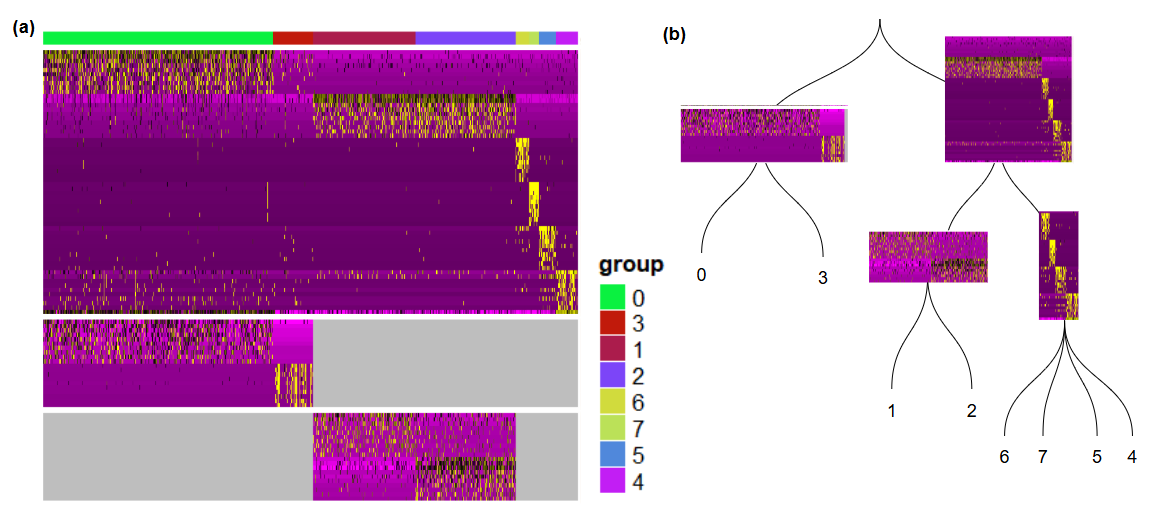
\includegraphics[width=0.75\linewidth]{additional_dataset_plot_hierarchy.png}
    \caption{\textbf{Overview of hierarchical marker gene selection in Activin A dataset.} \textbf{(a)} Assembled heatmap that concatenates marker gene heatmaps for individual splits in the constructed cell cluster hierarchy. \textbf{(b)} Our constructed hierarchical structure of cell clusters in the Activin A dataset.}
    \label{fig:Figure5}
\end{figure}

\section{Discussion}

Our analysis does not show that the Sun and Qiu method fails. On PBMC3k, the broad hierarchy remains stable across the parameter settings tested, and several marker-gene sets achieve good KNN classification performance. The more precise conclusion is that robustness depends on the level of analysis. The method can be stable at the hierarchy level, perform well at the classification level, and still be less stable at the marker-gene level.

This distinction is important for biological interpretation. If the goal is only to classify cells, different marker-gene lists may be sufficient. However, if the goal is to claim that specific genes characterize a lineage or cell type, then marker-gene stability becomes essential. Interpretability should therefore not only refer to a clear hierarchy or a readable heatmap, but also to the stability, compactness and biological meaning of the selected genes.

This result also connects with a criticism raised by Liu et al. regarding marker-gene selection: high classification performance is not sufficient if the selected gene set becomes too large or difficult to interpret \cite{liu2026}. Our results follow the same idea. The largest marker-gene set gives the highest mean KNN accuracy, but the improvement is limited and comes with many more genes. In contrast, smaller gene sets are easier to interpret biologically, but may lose some predictive power. This suggests that marker-gene selection should be evaluated not only by classification accuracy, but also by compactness and biological readability.


The main limitation of the original article is therefore not that its results are false. The central idea is sound, and the PBMC results support it. The limitation is that heatmap readability and classification accuracy do not fully test whether the same biological explanation is recovered across reasonable parameter choices. Our analysis adds this missing layer by comparing the stability of the hierarchy separately from the stability of the marker-gene lists.

There are also limitations in our analysis. Jaccard similarity measures gene overlap, but it does not show whether the strongest or most biologically informative markers are conserved. In addition, KNN accuracy is only one downstream classification metric, so further validation would be needed to evaluate biological robustness more completely.

% ------------------------------------------------------------

\addcontentsline{toc}{section}{References}

\begin{thebibliography}{9}

\bibitem{sun2024}
Sun, Y. and Qiu, P. (2024). \textit{Hierarchical marker genes selection in scRNA-seq analysis}. PLOS Computational Biology, 20(12): e1012643. \url{https://doi.org/10.1371/journal.pcbi.1012643}

\bibitem{liu2026}
Liu, Y., Baugh, A. G., Roussos Torres, E. T., and MacLean, A. L. (2026). \textit{Inference of marker genes of subtle cell state changes via iLR: iterative logistic regression}. Bioinformatics, 42(2): btag051. \url{https://doi.org/10.1093/bioinformatics/btag051}

\bibitem{yin2026}
Yin, W., et al. \textit{Activin a Secretion by Muscle-Repairing Macrophages Induces Heterotopic Ossification in Mice.} Journal of Clinical Investigation, vol. 136, no. 5, 2 Mar. 2026, \url{https://doi.org/10.1172/jci193797}.

\end{thebibliography}

\end{document}

